\section{Results}
\label{sec:results}

We tested our system against various datasets collected from the internet.
The first is a 1000-graph synthetic example dataset provided with the 
GraphGen utility. We also used two chamical compond databases available as
examples with several gSpan implementations (Compound\_422 and Chemical\_340),
and the MCF-7 breast cancer tumor description dataset.

Table~\ref{tab:synth} contains the runtime, speedup, and efficiency of runs
produced by our parallel gspan algorithm on a synthetic dataset with
a support of 0.05. The serial runtime is 76.95~seconds. By doubling
the number of processes we observe a decrease in runtime of 51.89. This
is due a speedup of 1.483. Further increasing the number of processes continues
to decrease the runtime, although the speedup continues to be suboptimal.
Figure~\ref{fig:synth} contains plots of runtime, speedup, and efficiency for
these runs. We clearly observe with these plots the decrease in runtime as the
number of processes increases. We also observe the degradation in speedup and
efficiency as the number of processes increases.


\begin{table}[H]
\centering
\begin{tabular}{cccc}
\hline
Cores & Runtime (seconds) & Speedup &  Eff.  \\
\hline
1    &   76.95   &  1.000 &     1.000  \\
2    &   51.89   &  1.483 &     0.741  \\
4    &   39.46   &  1.950 &     0.488  \\
8    &   31.36   &  2.454 &     0.307  \\
16   &   26.77   &  2.874 &     0.180  \\
32   &   24.15   &  3.186 &     0.100  \\
\hline
\end{tabular}
\caption{Runtime, speedup, and efficiency for synthetic dataset with support
         0.05.}
\label{tab:synth}
\end{table}

\begin{figure}[H]
\centering
\begin{tabular}{ccc}
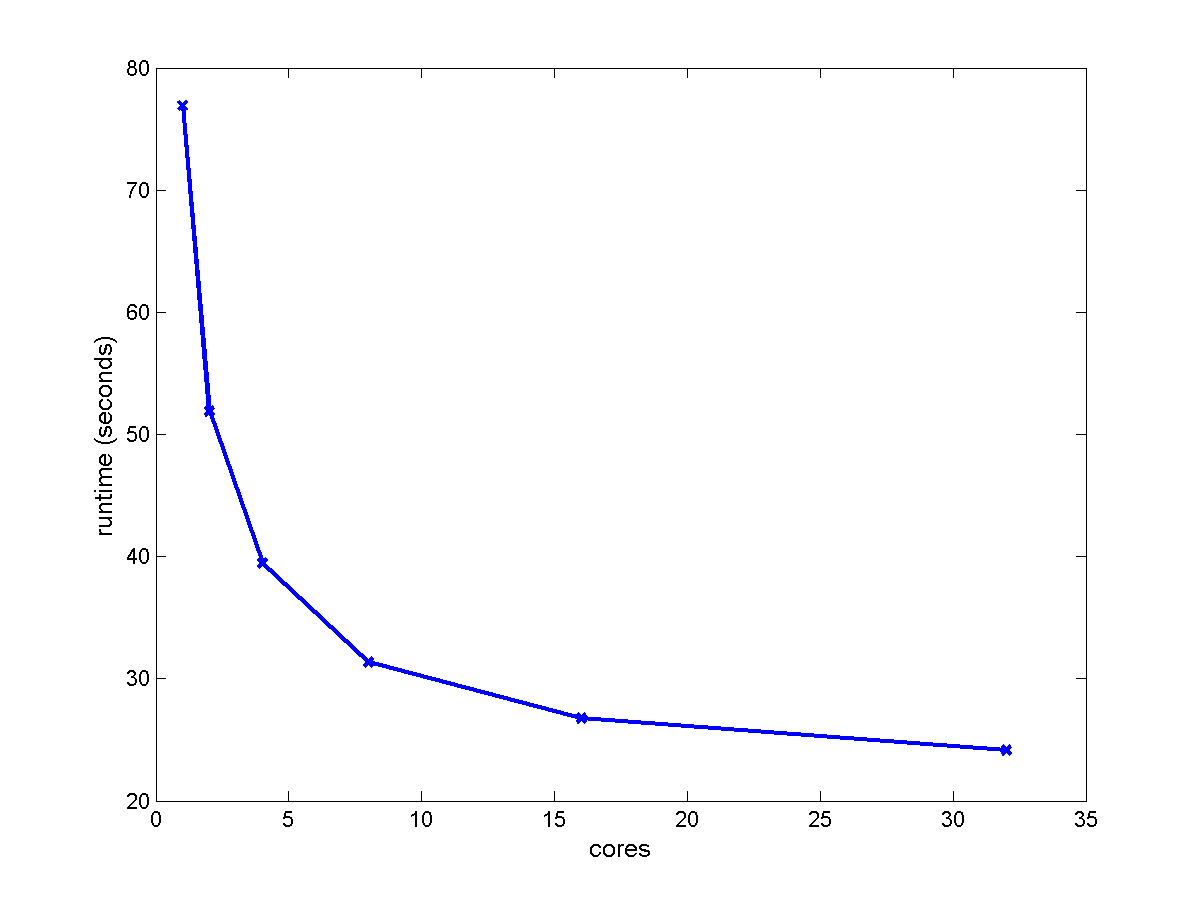
\includegraphics[width=0.3\textwidth]{synth_time.png} &
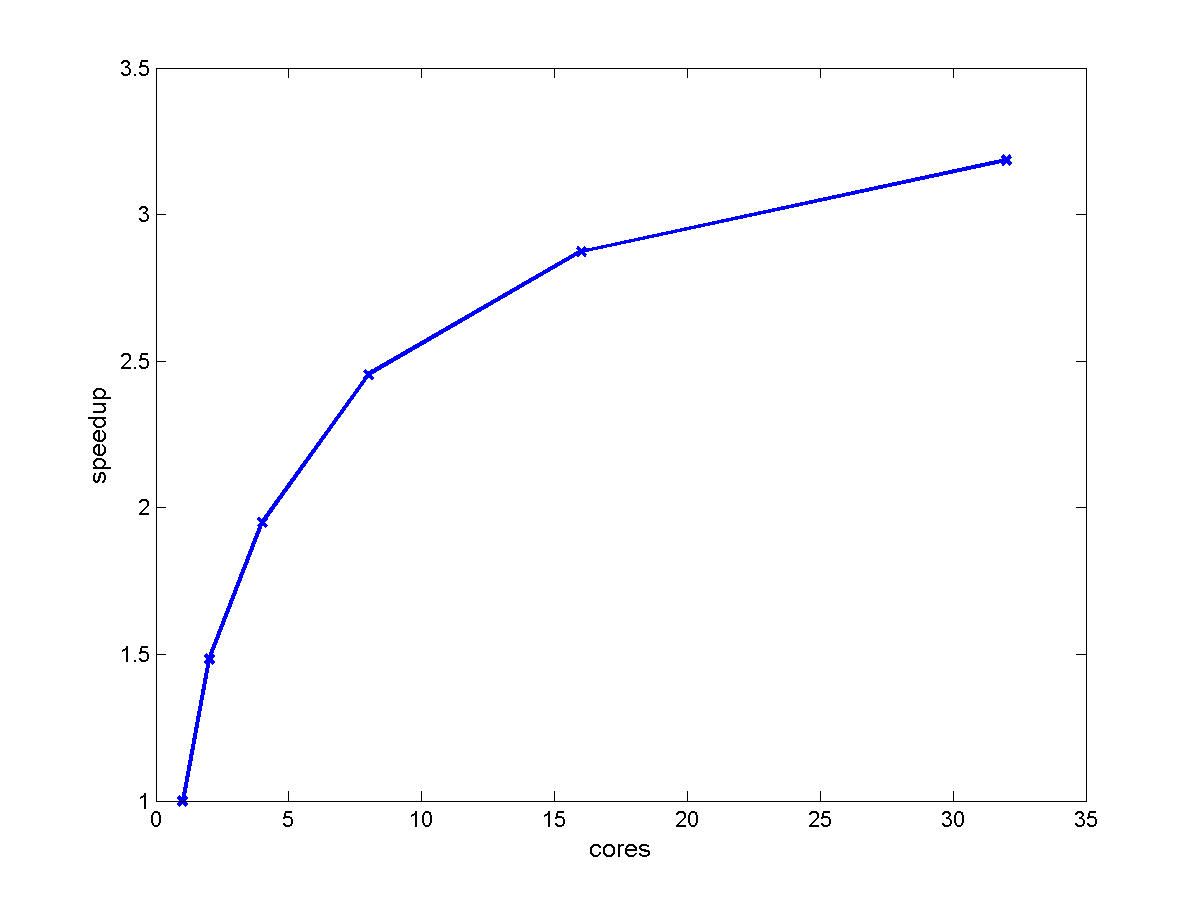
\includegraphics[width=0.3\textwidth]{synth_speedup.png} &
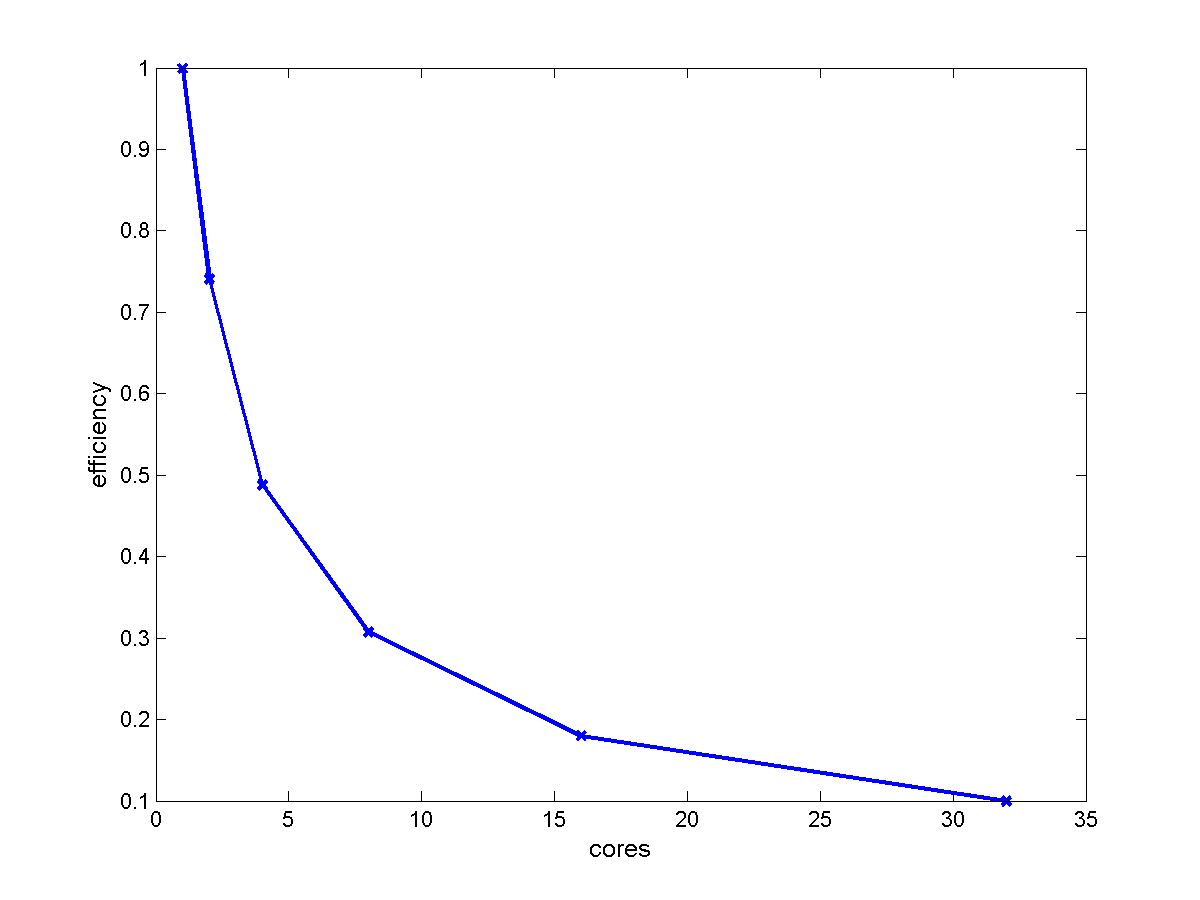
\includegraphics[width=0.3\textwidth]{synth_efficiency.png} \\
(a) & (b) & (c) \\
\end{tabular}
\caption{Plots of (a) runtime, (b) speedup, and (c) efficiency for
         synthetic dataset with support 0.05.}
\label{fig:synth}
\end{figure}

Table~\ref{tab:compound} contains results for the Compound\_422 dataset with
support of 0.1. We observe similar behavior as for the synthetic dataset. The
serial runtime for this dataset is 75.92~seconds. Doubling the number of
processes results in a runtime of 56.34. Doubling the number of processes again
to 4 processes results in a runtime 37.53~seconds. This is still a reasonable,
although suboptimal, speedup. However, if we increase the number of processes
to 8 processes we actually observe an increase in runtime to 40.97~seconds.
Further increasing the number of processes results in an insignificant decrease
in runtime.
Figure~\ref{fig:compound} contains plots of runtime, speedup, and efficiency
for these runs. The runtime plot clearly demonstrates the initial decrease in
runtime for smaller number of nodes, and the leveling off of the runtime for larger
numbers of nodes. We also observe the degradation in speedup and efficiency,
particularly for large numbers of nodes.


\begin{table}[H]
\centering
\begin{tabular}{cccc}
\hline
Cores & Runtime (seconds) & Speedup &  Eff.  \\
\hline
 1    &   75.92    &  1.000 & 1.000 \\
 2    &   56.34    &  1.348 & 0.674 \\
 4    &   37.53    &  2.023 & 0.506 \\
 8    &   40.97    &  1.853 & 0.232 \\
16    &   31.16    &  2.436 & 0.152 \\
32    &   32.08    &  2.367 & 0.074 \\
\hline
\end{tabular}
\caption{Runtime, speedup, and efficiency for Compound\_422 dataset with support
         0.1.}
\label{tab:compound}
\end{table}

\begin{figure}[H]
\centering
\begin{tabular}{ccc}
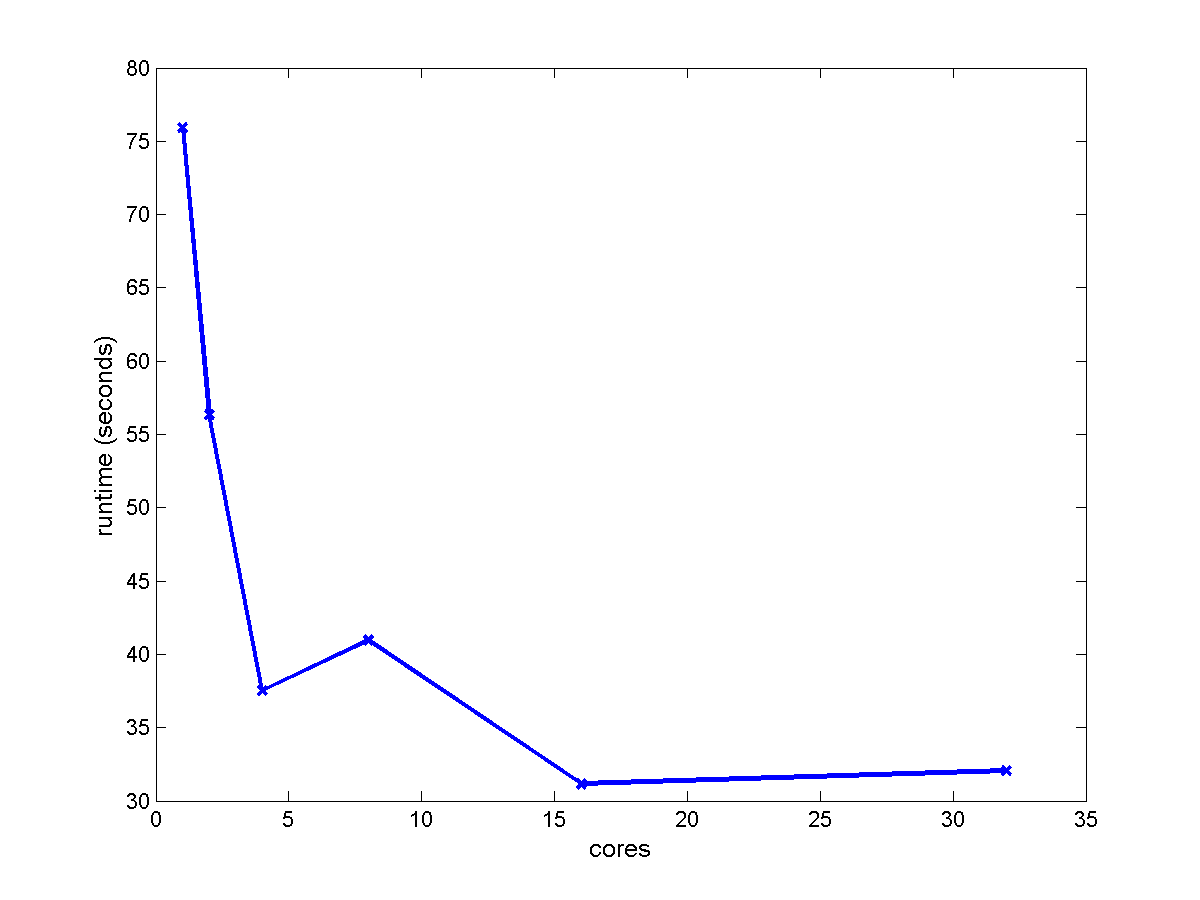
\includegraphics[width=0.3\textwidth]{compound_time.png} &
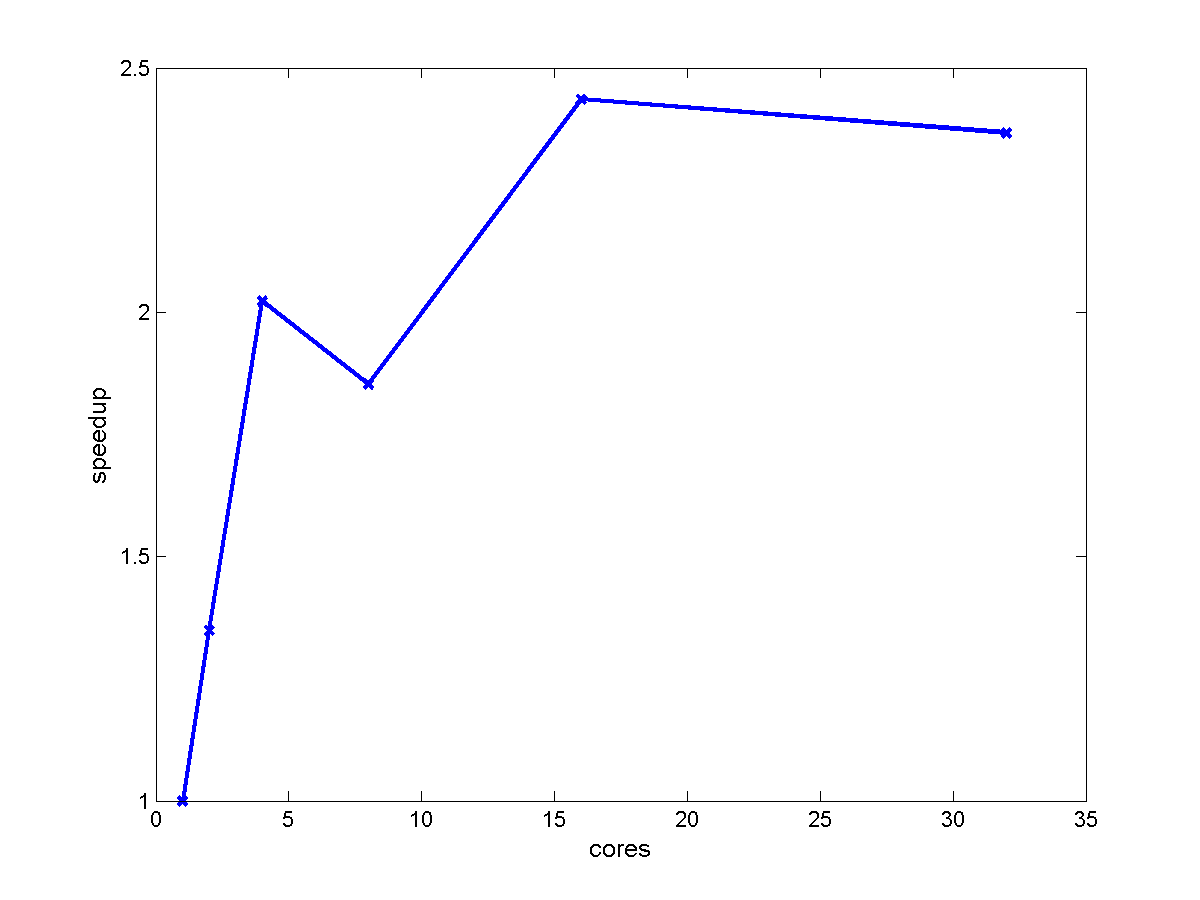
\includegraphics[width=0.3\textwidth]{compound_speedup.png} &
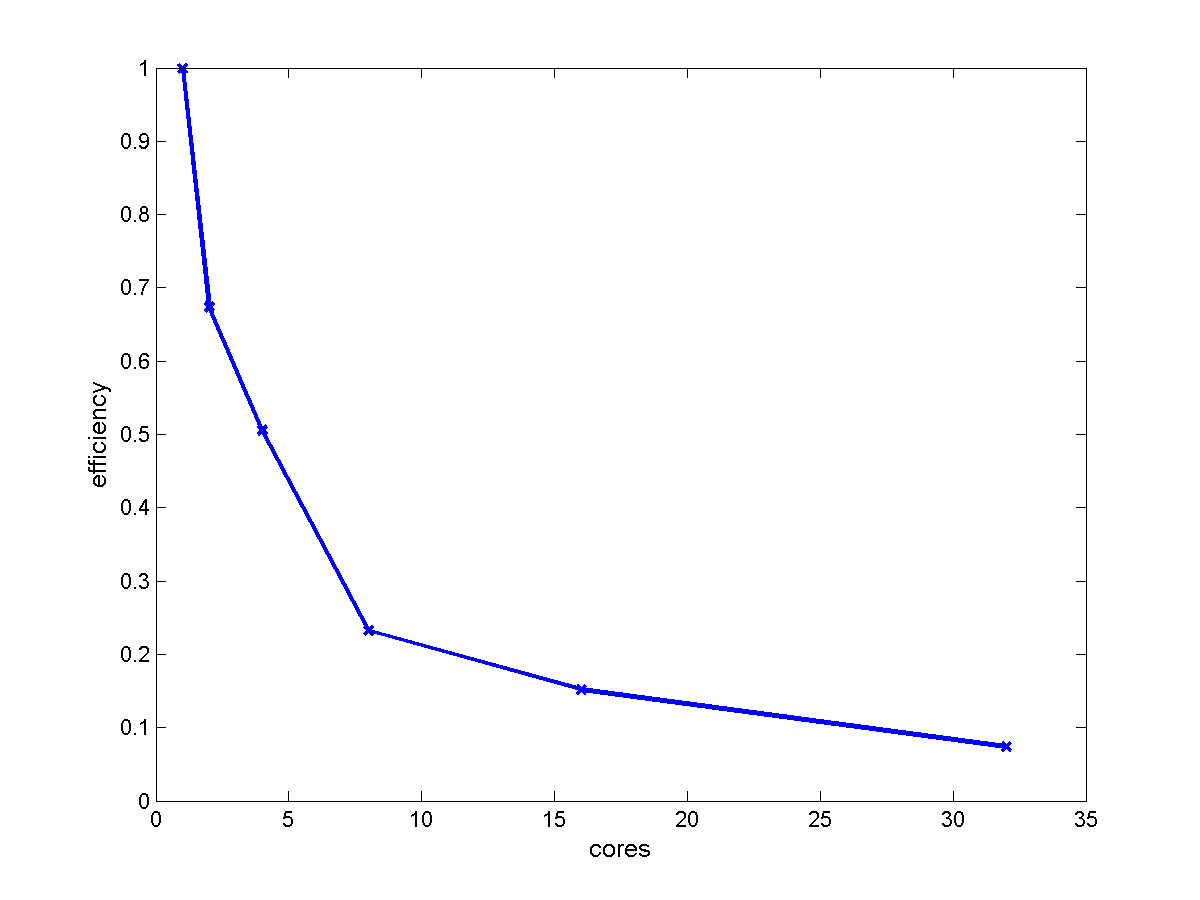
\includegraphics[width=0.3\textwidth]{compound_efficiency.png} \\
(a) & (b) & (c) \\
\end{tabular}
\caption{Plots of (a) runtime, (b) speedup, and (c) efficiency for
         Compound\_422 with support 0.1.}
\label{fig:compound}
\end{figure}

Table~\ref{tab:mcg7} contains results for the MCF-7 dataset with
support of 0.1. This dataset demonstrates the worst case results for our
method. The serial runtime for this dataset is 2503.03~seconds.
Doubling the number of processes results in a runtime of 2272.73~seconds. This
is a speedup of just 1.101 and efficiency of 0.551. Further doubling the number
of nodes decreases the runtime to 2239.04~seconds. This is a speedup of 1.118
and efficiency of 0.279. Doubling the number of processes again to 8 decreases
the runtime to 2061.45~seconds. This is a speedup of 1.214 and efficiency of
0.152. Any further increases in processes result in an increase in runtime.
Figure~\ref{fig:mcg7} contains plots of runtime, speedup, and efficiency
for these runs. The runtime plot clearly demonstrates the poor performance of
our code on multiple nodes for this dataset. We observe that the speedup and
efficiency quickly deteriorate.


\begin{table}[H]
\centering
\begin{tabular}{cccc}
\hline
Cores & Runtime (seconds) & Speedup &  Eff.  \\
\hline
 1    & 2503.03 & 1.000  & 1.000 \\
 2    & 2272.73 & 1.101  & 0.551 \\
 4    & 2239.04 & 1.118  & 0.279 \\
 8    & 2061.45 & 1.214  & 0.152 \\
16    & 2234.83 & 1.120  & 0.070 \\
32    & 2234.83 & 1.142  & 0.036 \\
\hline
\end{tabular}
\caption{Runtime, speedup, and efficiency for MCF-7 with support
         0.1.}
\label{tab:mcg7}
\end{table}

\begin{figure}[H]
\centering
\begin{tabular}{ccc}
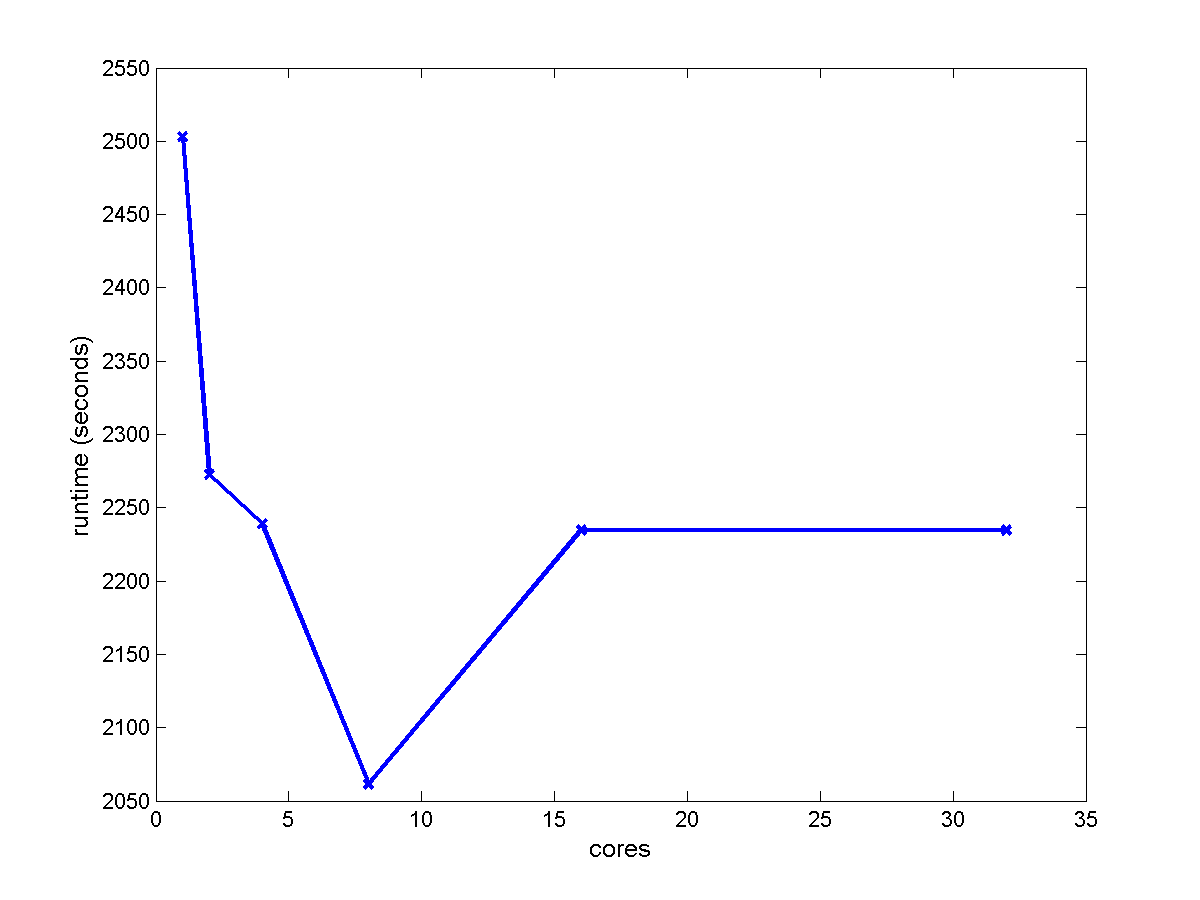
\includegraphics[width=0.3\textwidth]{mcg7_time.png} &
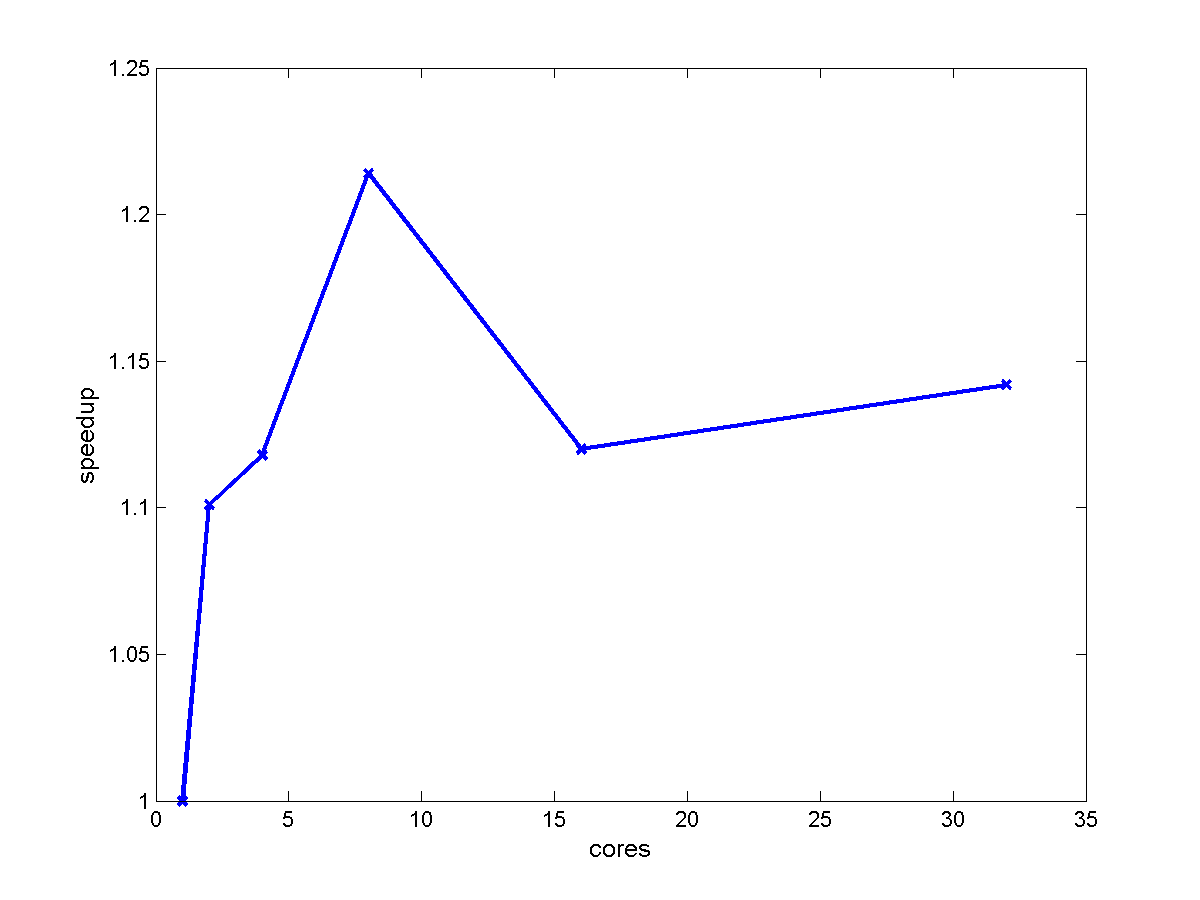
\includegraphics[width=0.3\textwidth]{mcg7_speedup.png} &
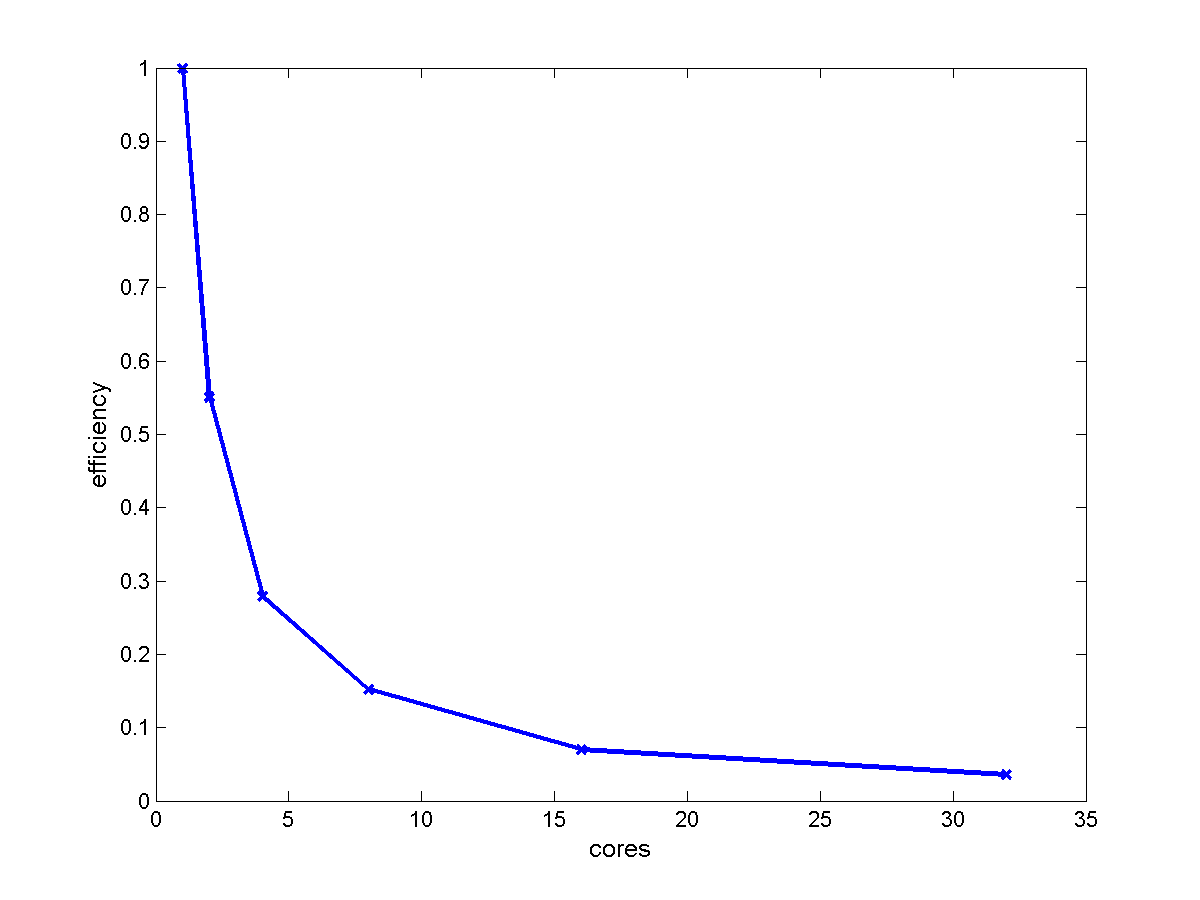
\includegraphics[width=0.3\textwidth]{mcg7_efficiency.png} \\
(a) & (b) & (c) \\
\end{tabular}
\caption{Plots of (a) runtime, (b) speedup, and (c) efficiency for
         MCF-7 with support 0.1.}
\label{fig:mcg7}
\end{figure}


During these runs we found that
for the synthetic dataset one of the edges takes 3.026~seconds to mine,
for the Compound\_422 dataset one of the edges takes 31.157~seconds to mine,
and for the MCF-7 dataset one of the edges takes 2060.85~seconds to mine.
Since our method parallelizes the algorithm by splitting up the edges between
MPI processes we cannot perform any faster than it takes to
mine the slowest edge.
We can see that for the Compound\_422 and MCF-7 datasets our overall runtime
is very close to the runtime of the slowest edge. For the Compound\_422
dataset, for instance, a runtime of 31.16~seconds is achieved with
16~processes. Since the slowest edge takes 31.157~seconds it is not surprising
that increasing the number of processes 32 increases the runtime. Since the
serial time is only 75.92~seconds and we cannot have a runtime lower than
31.16~seconds this explains our poor speedup.
The MCF-7 dataset demonstrates this issue more clearly. Our serial runtime
is 2503.03~seconds and the slowest edge takes 2060.85~seconds. This means
that no matter how many processes we use it is not possible to even halve
our runtime. In fact, we can achieve very close to this runtime for our
overall code when using 8~processes.
However, the synthetic dataset has a serial runtime of 76.95~seconds and
the slowest edge takes 3.026~seconds to mine. For such a dataset it should
be possible to get good performance using our method. However, using
32~processes only gives us a runtime of 24.15~seconds.

As described in more detail in Section~\ref{sec:implementation}, the method
which we implemented for these results statically partitions the edges between
the processes and each process independently mines each of its edges. The
results in Table~\ref{tab:synth_dyn} contain results for a method that uses a
centralized dynamic load balancing to allocate edges among the processes
using the synthetic dataset. We do not include results for the
Compound\_422 and MCF-7 datasets as we have shown that our method
cannot perform any better due to the time it takes to mine the slowest edge.
The hope is that this more evenly
distributes the work between the processes. In this method process 0 will
contain a counter with the next edge that needs to be mined. All other
processes will mine an edge. Once a process finishes mining an edge it will
send a message to process 0 telling it that it is finished. If there are still
edges to be mined process 0 sends the id of the next edge.

The first column of
Table~\ref{tab:synth_dyn} contains the number of worker processes used, the
second column contains the runtime, the third column contains the speedup, and
the fourth column contains the efficiency.  We observe a small increase in
runtime using 1 and 2 processes due to the increase in communication between
processes. However, for larger numbers of processes there is an improvement in
runtime using this method for the previous static method. However, the
improvement is not significant and the we observe all modest improvements in
speedup and efficiency over the previous method. For instance, using 32
processes we now have a speedup of 4.845 and efficiency of 0.151, compared to
the previous speedup of 3.186 and efficiency of 0.100. Although this is an
improvement, our speedup and efficiency are still suboptimal. This can be
explained by the increased MPI communication between processes. After an edge
is mined, two messages are sent from the finished process to process 0,
compared to no communication required in the static implementation.


\begin{table}[H]
\centering
\begin{tabular}{cccc}
\hline
Cores & Runtime (seconds) & Speedup &  Eff.  \\
\hline
1   &    87.40   &     1.000  &    1.000   \\ 
2   &    53.89   &     1.622  &    0.811   \\
4   &    32.70   &     2.673  &    0.668   \\
8   &    26.37   &     3.314  &    0.414   \\
16  &    21.21   &     4.121  &    0.258   \\
32  &    18.04   &     4.845  &    0.151   \\
\hline
\end{tabular}
\caption{Runtime, speedup, and efficiency for synthetic dataset with support
         0.05 using centralized dynamic load balancing.}
\label{tab:synth_dyn}
\end{table}

\begin{figure}[H]
\centering
\begin{tabular}{ccc}
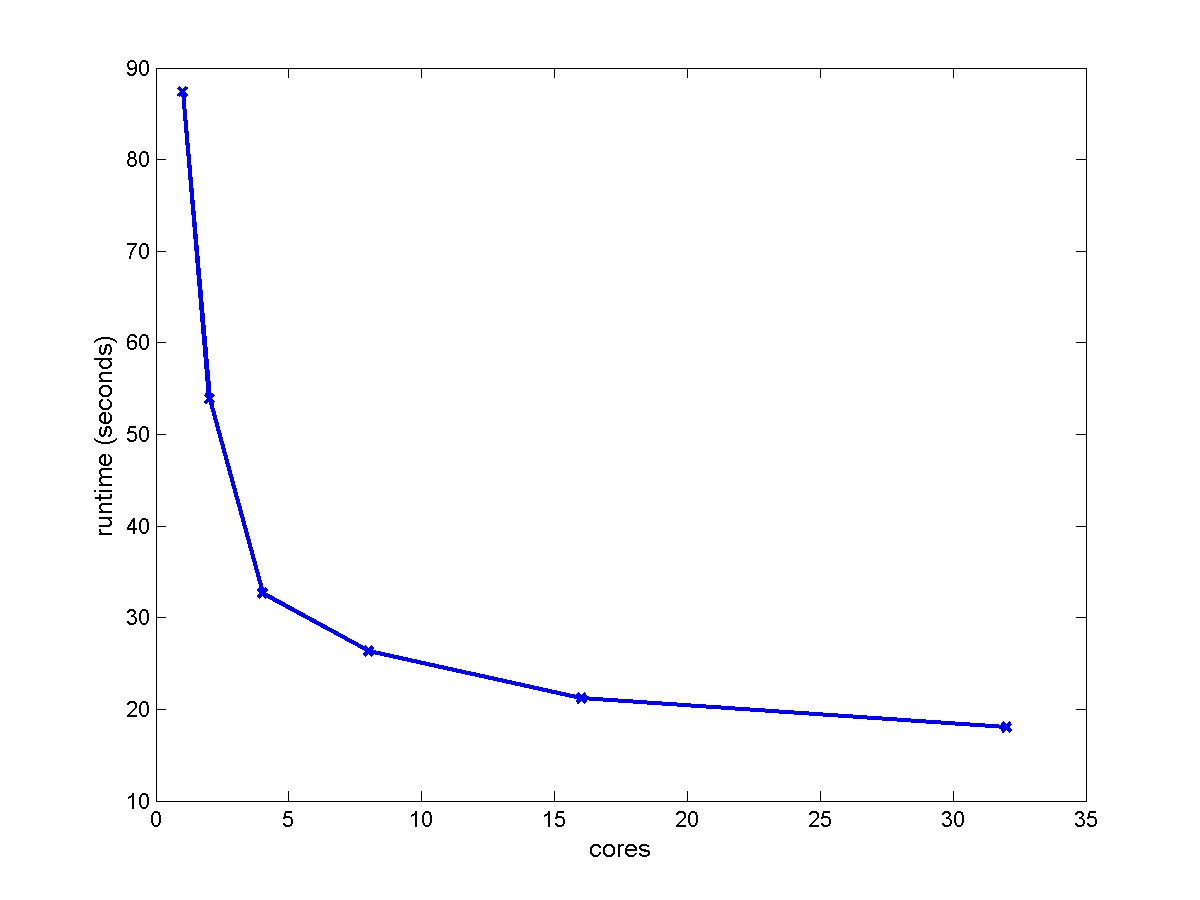
\includegraphics[width=0.3\textwidth]{synth_dyn_time.png} &
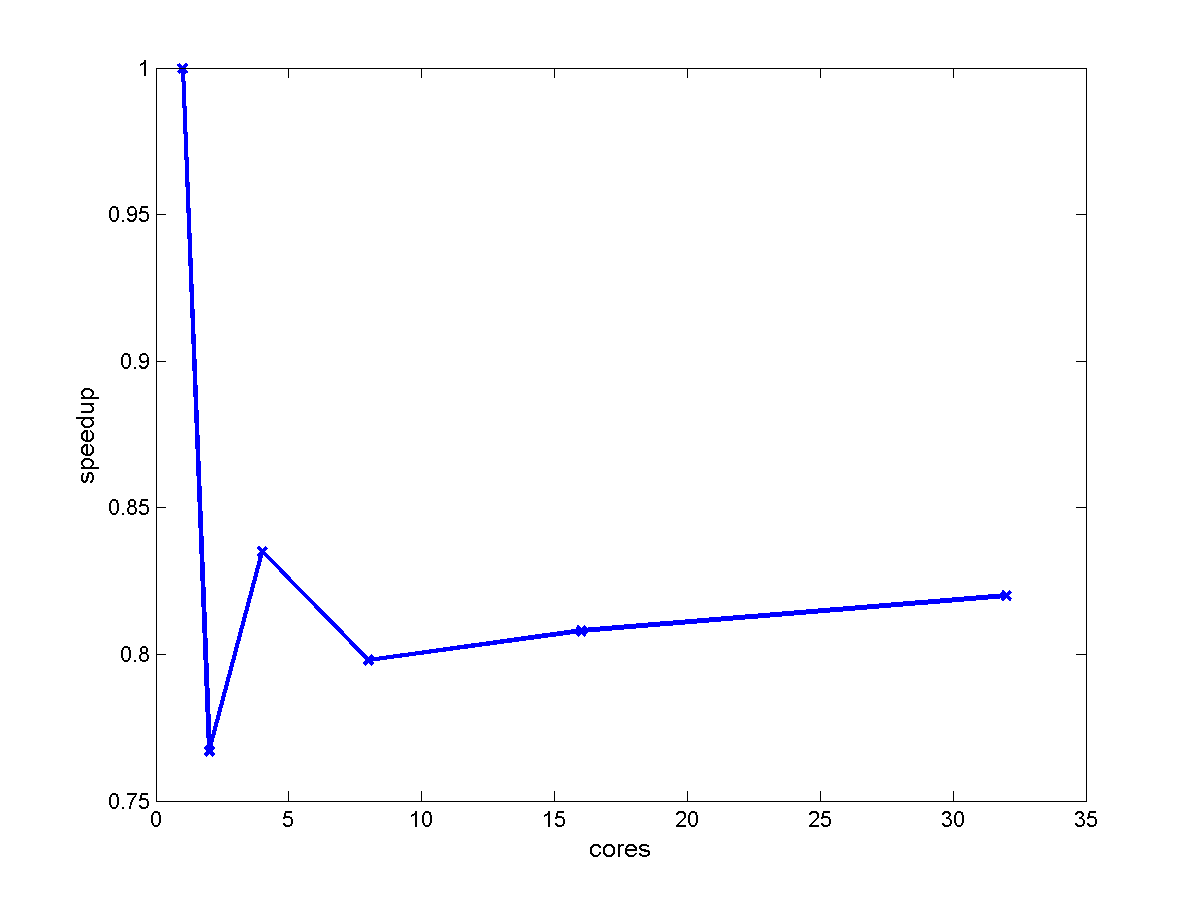
\includegraphics[width=0.3\textwidth]{synth_dyn_speedup.png} &
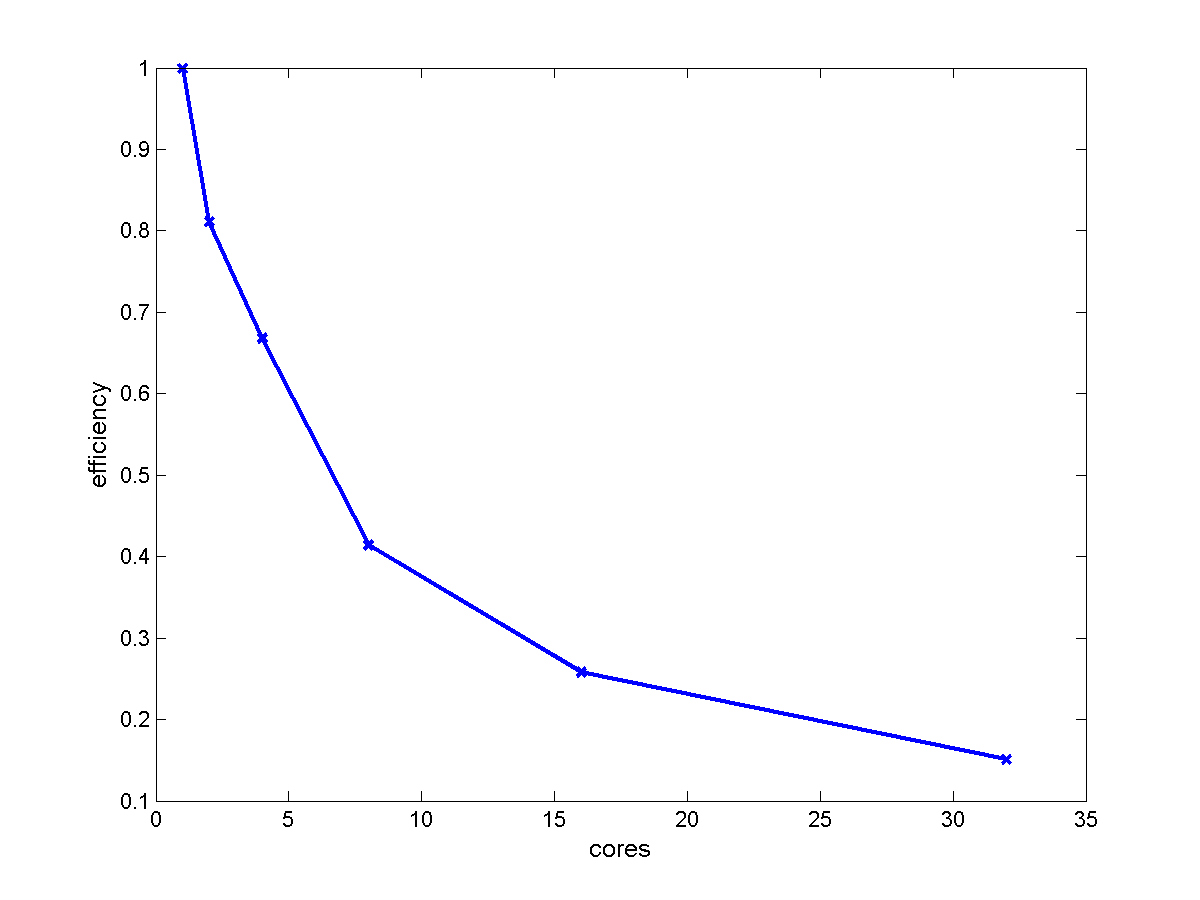
\includegraphics[width=0.3\textwidth]{synth_dyn_efficiency.png} \\
(a) & (b) & (c) \\
\end{tabular}
\caption{Plots of (a) runtime, (b) speedup, and (c) efficiency for
         synthetic dataset with support 0.05 centralized dynamic load
         balancing.}
\label{fig:synth_dyn}
\end{figure}

%\begin{table}
%\centering
%\begin{tabular}{cccc}
%\hline
%Cores & Runtime (seconds) & Speedup &  Eff.  \\
%\hline
%1   & 71.44 &       &       \\
%2   & 35.41 &       &       \\
%4   & 32.87 &       &       \\
%8   & 32.36 &       &       \\
%16  & 30.59 &       &       \\
%32  &       &       &       \\
%\hline
%\end{tabular}
%\caption{Runtime, speedup, and efficiency for Compound\_422 dataset with
%         support 0.1 using centralized dynamic load balancing.}
%\label{tab:compound_dyn}
%\end{table}

%\begin{table}
%\centering
%\begin{tabular}{cccc}
%\hline
%Cores & Runtime (seconds) & Speedup &  Eff.  \\
%\hline
%1   &  &       &       \\
%2   &  &       &       \\
%4   & 2201.26 &       &       \\
%8   & 2228.37 &       &       \\
%16  &  &       &       \\
%32  &  &       &       \\
%\hline
%\end{tabular}
%\caption{Runtime, speedup, and efficiency for MCG-7 dataset with
%         support 0.1 using centralized dynamic load balancing.}
%\label{tab:mcg_dyn}
%\end{table}
